\newpage
\subsection{Declaring classes and attributes}
\texHeader
\hypertarget{static:classes tex}{}

% Discuss syntax in this section! (We removed it from Part I)
\begin{itemize}

\item[$\blacktriangleright$] Right click \texttt{LearningBoxLanguage}, and create your first EClass by choosing ``New/EClass.'' Name it \texttt{Box}.

\item[$\blacktriangleright$] The class editor should automatically open. Let's add the first two EAttributes of our program, \texttt{name} and
\texttt{stringRep}. In MOSL, attributes are declared by stating their name and type as \texttt{name:type}. In this case, both are of type \texttt{EString}
(Fig.~\ref{fig:boxDeclaration}).

\vspace{0.5cm}

\begin{figure}[htbp]
	\centering
  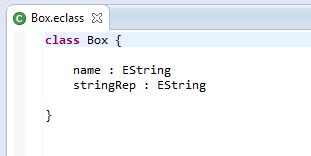
\includegraphics[width=0.5\textwidth]{eclipse_classBoxDeclaration}
	\caption{Newly created box class}
	\label{fig:boxDeclaration}
\end{figure} 

\vspace{0.5cm}

\item[$\blacktriangleright$] Create two empty classes in your model, \texttt{Partition} and \texttt{Card}.

\item[$\blacktriangleright$] In \texttt{Partition}, add two \texttt{EInt} attributes, \texttt{index} and \texttt{partitionSize}.

\item[$\blacktriangleright$] In \texttt{Card}, create three \texttt{EString} attributes, \texttt{back}, \texttt{face} , and \texttt{partitionHistory}.

\item[$\blacktriangleright$] If you've done everything correctly, your workspace should now resemble Fig.~\ref{fig:workspaceClassAttributes}.

\item[$\blacktriangleright$] That's it for declaring class attributes! Feel free to build your project again and view the changes in the \texttt{.ecore}
mode, and the generated files in ``gen" and ``src." On a final note, while some languages (such as Java) allow the declaration of several small classes (such as
these three) in the same file, when tooling with eMolfon, we keep them separated. Don't worry - we'll explain this later in the handbook. As for now, continue
to the next section to start creating references between these classes.

\newpage

\vspace*{3cm}

\begin{figure}[htbp]
	\centering
  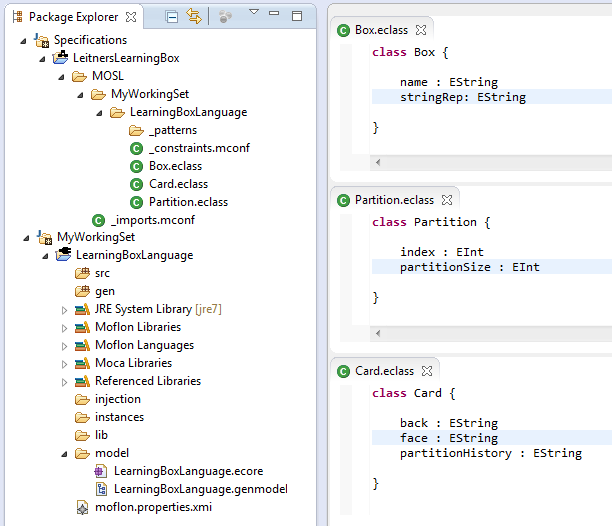
\includegraphics[width=1.0\textwidth]{eclipse_workspaceTexClassAttributes}
	\caption{Declaration of classes and attributes}
	\label{fig:workspaceClassAttributes}
\end{figure} 

% \fancyfoot[R]{$\triangleright$ \hyperlink{static:references splash}{Next}}

\end{itemize}
